% =============================================================================
%  Packages and document-wide settings.
%
%  Kept separate from main.tex so a university template can replace the class
%  and title page without touching this file, or replace this file wholesale
%  without touching any chapter.
% =============================================================================

% --- Encoding and language ----------------------------------------------------
\usepackage[T1]{fontenc}
\usepackage[utf8]{inputenc}
\usepackage[english]{babel}
\usepackage{csquotes}          % required by biblatex; also gives \enquote{}
\usepackage{microtype}         % subtle spacing/protrusion — noticeably better justification

% --- Maths --------------------------------------------------------------------
\usepackage{amsmath}
\usepackage{amssymb}

% --- Figures and tables -------------------------------------------------------
\usepackage{graphicx}
\graphicspath{{figures/}}      % so 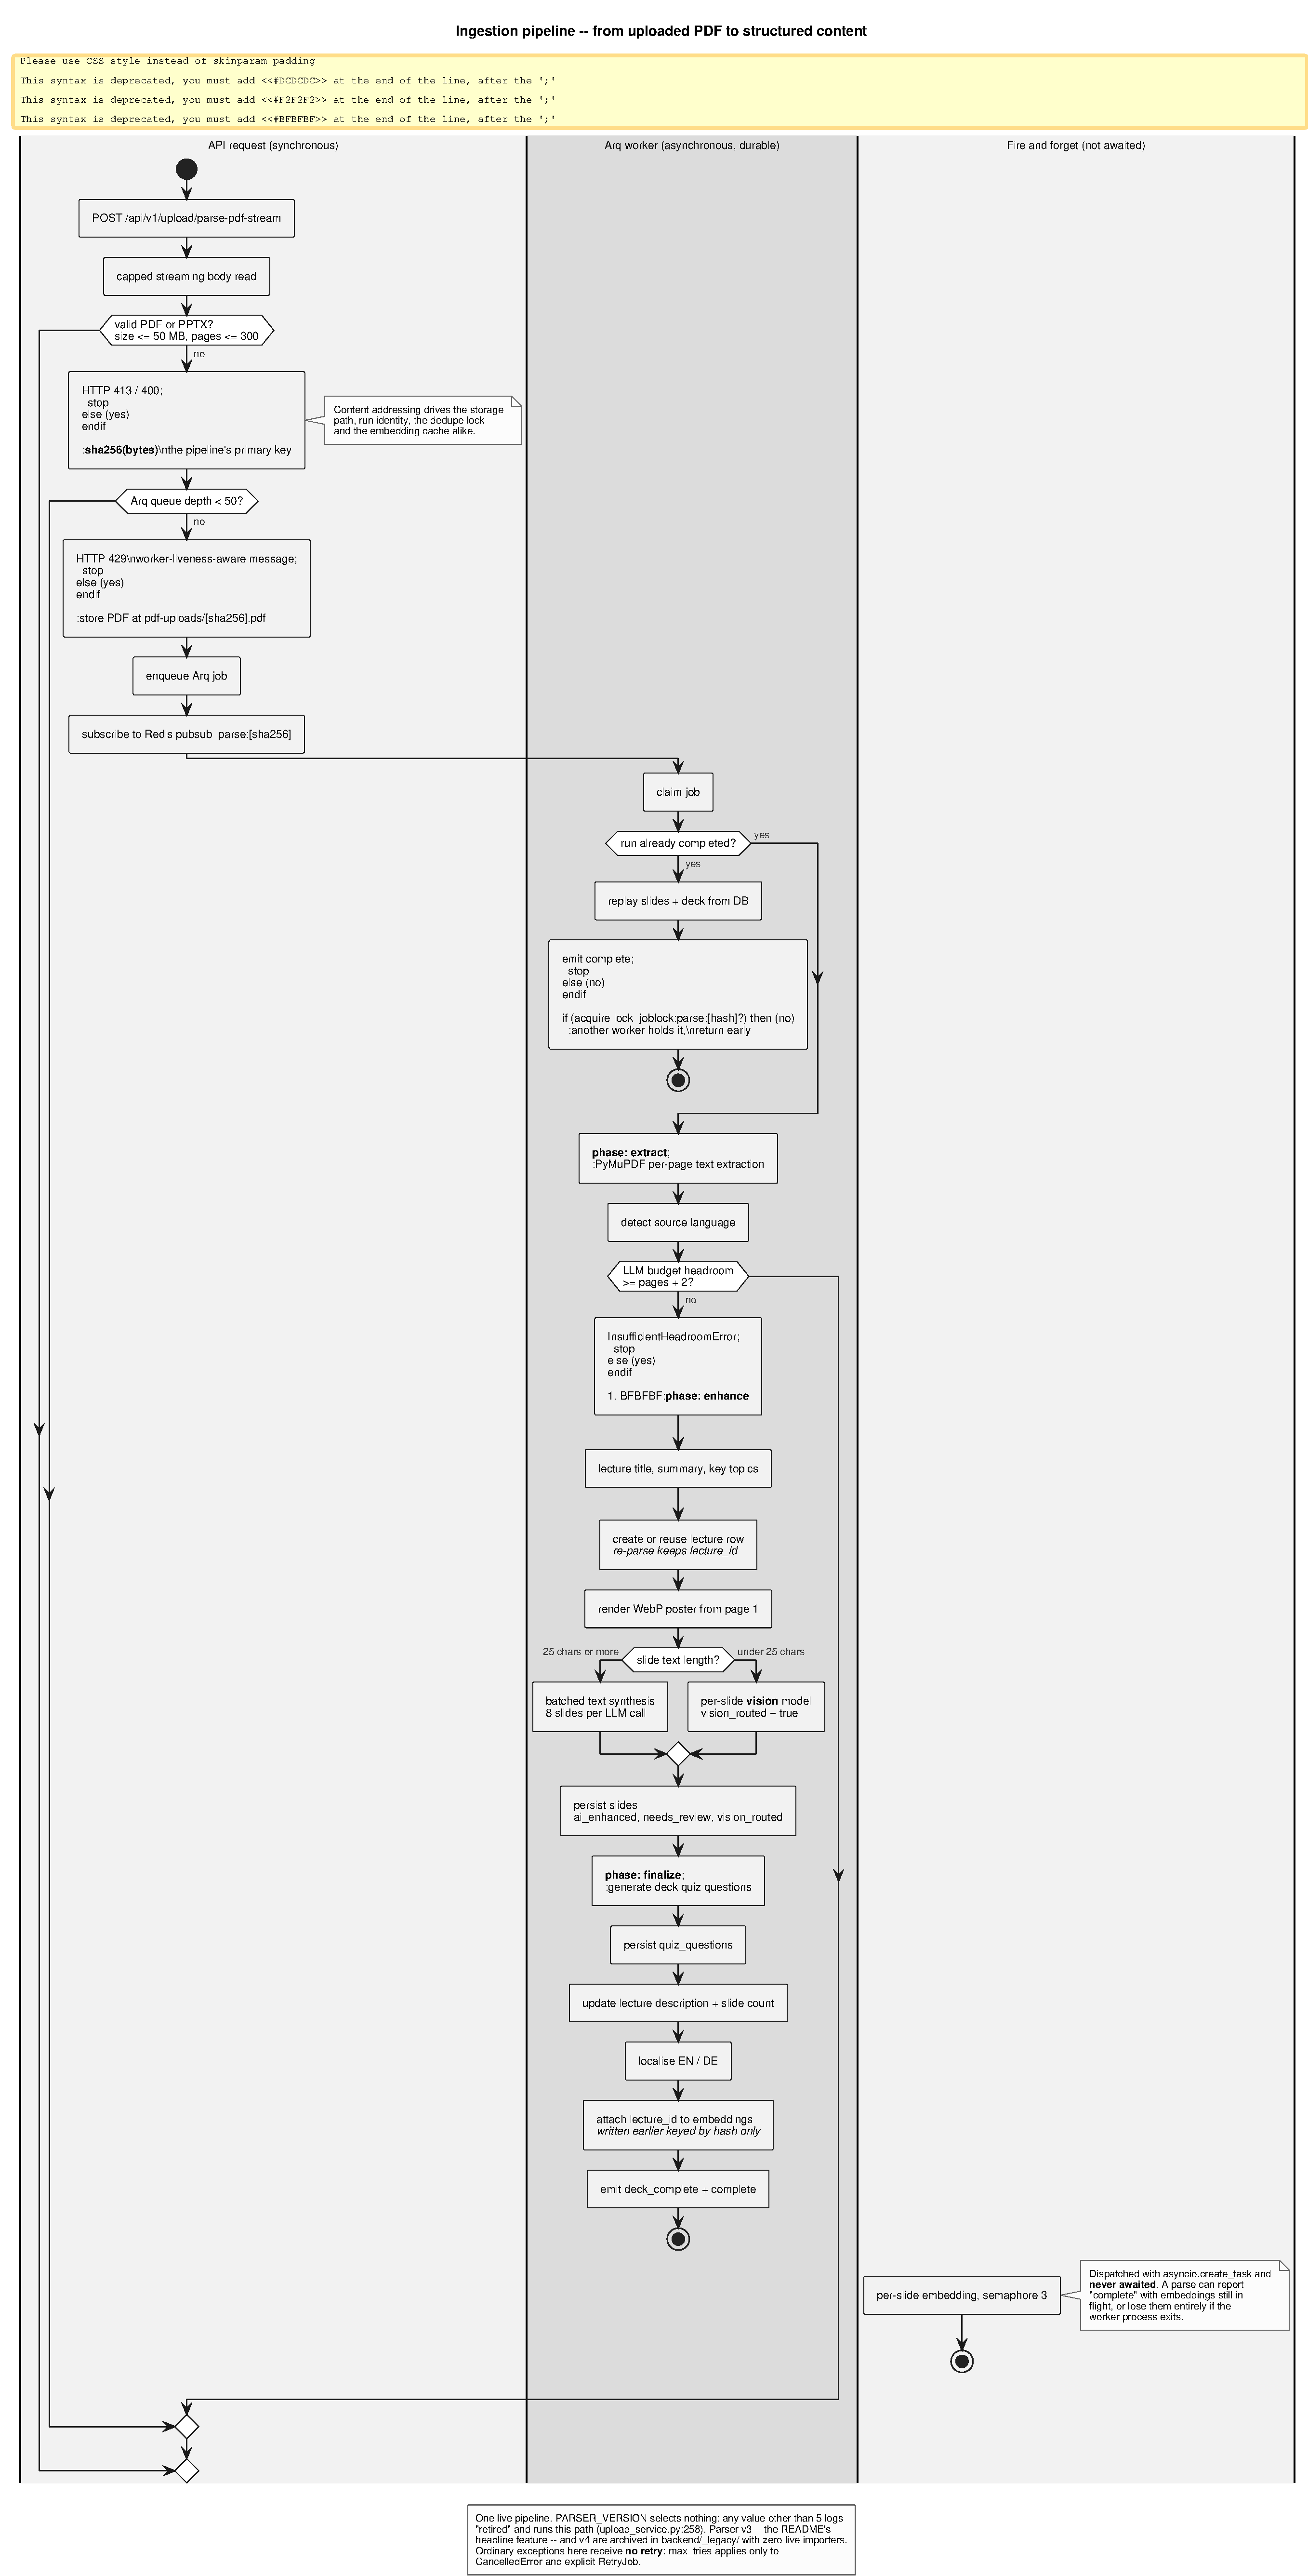
\includegraphics{f8-pipeline} just works
\usepackage{booktabs}          % \toprule/\midrule/\bottomrule — no vertical rules
\usepackage{longtable}         % tables that span pages (the honesty ledger will)
\usepackage{float}
\usepackage[export]{adjustbox} % lets a too-wide figure be scaled in place

% IMPORTANT — PDF 2.0 figure inclusion.
% The PlantUML-generated figures are PDF 2.0. pdfTeX refuses to \includegraphics
% a PDF whose version exceeds its own output version, failing with
%   "PDF inclusion: found PDF version <2.0>, but at most version <1.7> allowed".
% Raising the output version fixes it on TeX Live 2023+. \pdfvariable is
% undefined on older engines, hence the guard.
%
% If you still hit that error, switch the figure pipeline to EPS: set
%   PDF_FLAG = -teps
% in figures/Makefile and add an epstopdf step (epstopdf ships with TeX Live).
\ifdefined\pdfvariable
  \pdfvariable majorversion=2
  \pdfvariable minorversion=0
\fi

% --- Code listings ------------------------------------------------------------
\usepackage{listings}
\lstset{
  basicstyle=\ttfamily\footnotesize,
  breaklines=true,
  captionpos=b,
  frame=single,
  showstringspaces=false,
  numbers=left,
  numberstyle=\tiny\color{gray},
  keywordstyle=\bfseries,
  commentstyle=\itshape\color{gray},
  columns=fullflexible,
}
\usepackage{xcolor}

% --- Bibliography -------------------------------------------------------------
% numeric-comp compresses [1,2,3] into [1-3]. Swap style= if your institute
% mandates author-year (e.g. style=authoryear).
\usepackage[
  backend=biber,
  style=numeric-comp,
  sorting=nyt,
  maxbibnames=99,
  giveninits=true,
]{biblatex}
\addbibresource{references.bib}

% --- Cross-references (load hyperref late, cleveref last) ---------------------
\usepackage[
  hidelinks,                   % no coloured boxes — correct for a printed thesis
  pdfusetitle,
]{hyperref}
\usepackage[capitalise,noabbrev]{cleveref}

% --- Convenience --------------------------------------------------------------

% Standard figure inclusion. Usage:
%   \thesisfigure{f8-pipeline}{Ingestion pipeline, five observable phases.}{fig:pipeline}
% The figures are tall and narrow or wide and short depending on type, so width
% is capped at \textwidth and height at 0.85\textheight; whichever binds first
% wins, and nothing overflows the page.
\newcommand{\thesisfigure}[3]{%
  \begin{figure}[htbp]
    \centering
    \includegraphics[width=\textwidth,height=0.85\textheight,keepaspectratio]{#1}%
    \caption{#2}%
    \label{#3}%
  \end{figure}%
}

% Same, but for a figure that needs a full page of its own (the ER diagram and
% the tutor sequence diagram will).
\newcommand{\thesisfigurepage}[3]{%
  \begin{figure}[p]
    \centering
    \includegraphics[width=\textwidth,height=0.92\textheight,keepaspectratio]{#1}%
    \caption{#2}%
    \label{#3}%
  \end{figure}%
}

% Inline reference to a source location, e.g. \code{tutor.py:275}.
\newcommand{\code}[1]{\texttt{\small #1}}

% Visible TODO marker. Set \todosoff in metadata.tex before submitting to make
% every one of these vanish — then check the PDF for holes.
\newcommand{\TODO}[1]{\textcolor{red}{\textbf{[TODO: #1]}}}
\newcommand{\todosoff}{\renewcommand{\TODO}[1]{}}
